\chapter{Results} \label{chap:results}

This chapter contains waveforms and plots of the tests realized to determine the driving ability of the \ac{WMU} and their explanations. The tests were realized by applying two types of driving methods: Trapezoidal and sinusoidal drive. Both driving methods were tested under two conditions: loaded and unloaded. 

The load used for the loaded tests was a DC voltage generator attached to the HUB in-wheel motor. The generator acted as a load by attaching a small resistance to its terminals. The torque of the generator could be regulated by changing the field excitation voltage. The torque was measured with a load cell that was attached to the “floating” stator (how is this configuration named?). The deformation of the load cell was translated into a voltage signal by using the instrumentation amplifier HX711, which has a serial interface used to transfer the measured voltage which was later translated into torque by an Arduino Mega, used as an interface with a computer to read the torque applied for the following tests.

The power was supplied by a PeakTech (?) power supply with a voltage range up to 30 V and a current limit at 10 A. The voltage of the tests was 24 V.
All the control parameters of the test were modified and obtained “on-the-run” with a user interface developed in LabView.

\section{Trapezoidal Drive - Open Loop}

The trapezoidal waveform of the phase voltage on the motor was obtained by applying a six-step sequence drive on the windings of the motor, applying a \ac{PWM} on each phase commutating from $V_{DS}$ to $0V$.

Driving Frequency

\begin{figure}[htbp]
\centering
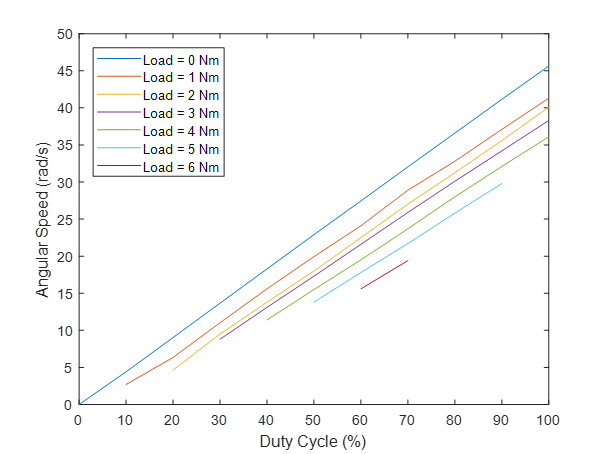
\includegraphics[width=10cm]{Images/plots/plot_1.png} 
\caption[plot1]{Plot of the different speeds achieved applying a known duty cycle using an open loop trapezoidal drive with different loads}
\label{fig:plot1}
\end{figure}

Figure \ref{fig:plot1} shows the different speeds achievable by applying different duty cycles to the six-step drive sequence with different torque loads. The curves on the plot start on different duty cycles since the torque load couldn’t reach a steady value until a certain speed was stablished. For example, for the measurement with a load equal to $3 Nm$, the curve starts at a duty cycle equal to $30\%$, since at a duty cycle lower than this or a speed lower than $10 rad/s$, the load can’t be generated by the test bench, which would give $2 Nm$ for example, therefore those measurements were not considered for the plot. On the other hand, the curves that don’t show large duty cycle values ($5$ and $6 Nm$), is because the power supply couldn’t feed enough current to the driver to reach such torque.

\subsection{Voltage Waveforms}

The following images show the different voltage waveforms obtained according to the load applied to the motor and to the duty cycle.

\begin{figure}[h!p]
\centering
	\subfloat[Duty Cycle = 10\%\label{subfig-1:trap1}]{%
  		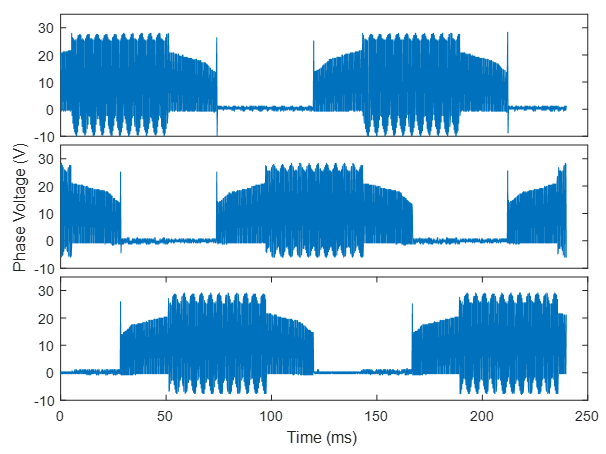
\includegraphics[clip,width=8cm]{Images/waveforms/trap_1.png}%
	}

	\subfloat[Duty Cycle = 50\%\label{subfig-2:trap2}]{%
  		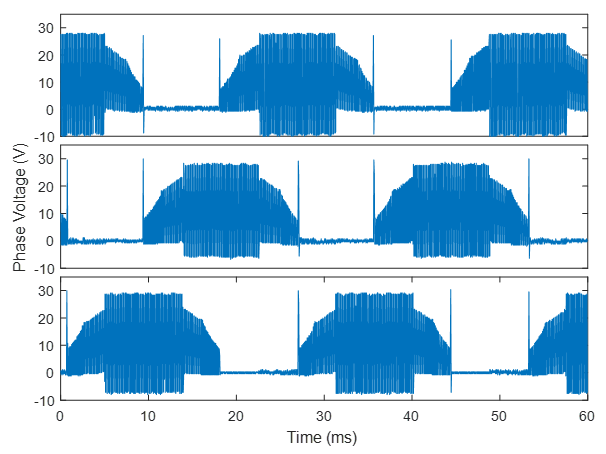
\includegraphics[clip,width=8cm]{Images/waveforms/trap_2.png}%
	}

	\subfloat[Duty Cycle = 100\%\label{subfig-3:trap3}]{%
  		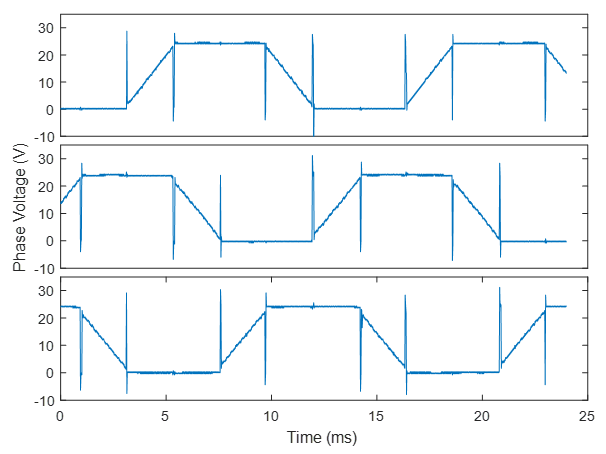
\includegraphics[clip,width=8cm]{Images/waveforms/trap_3.png}%
	}
\caption{Trapezoidal drive without load applied}
\end{figure}



\begin{figure}[h!p]
\centering
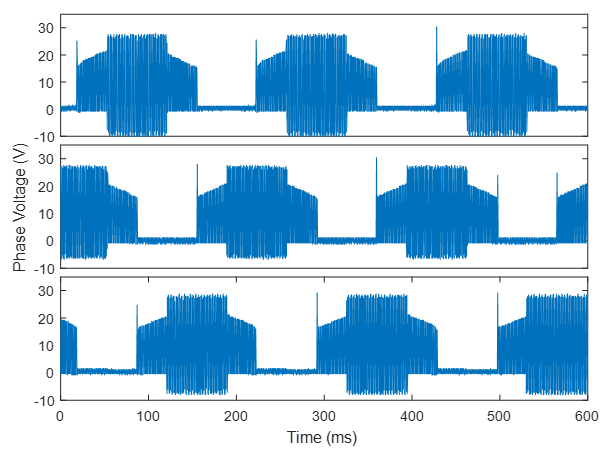
\includegraphics[width=10cm]{Images/waveforms/trap_4.png} 
\caption[trap4]{Duty Cycle = 10\%, load = 1 Nm}
\label{fig:trap4}
\end{figure}

\begin{figure}[h!p]
\centering
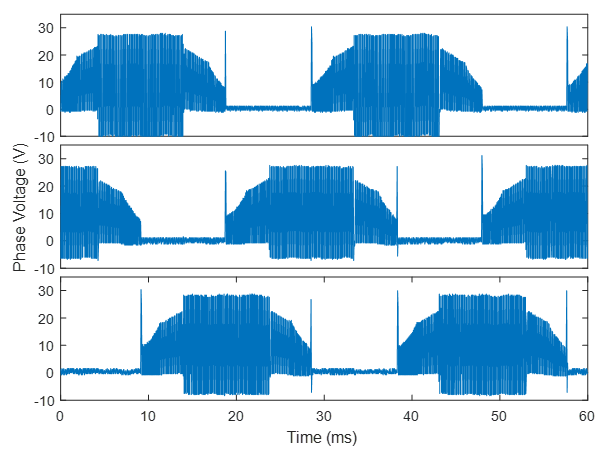
\includegraphics[width=10cm]{Images/waveforms/trap_5.png} 
\caption[trap5]{Duty Cycle = 50\%, load = 1 Nm}
\label{fig:trap5}
\end{figure}

\begin{figure}[h!p]
\centering
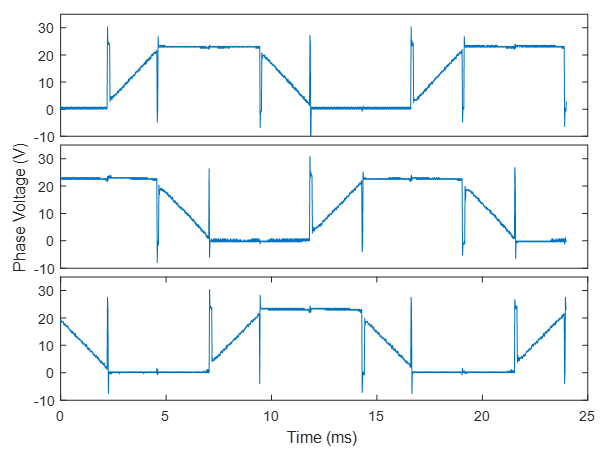
\includegraphics[width=10cm]{Images/waveforms/trap_6.png} 
\caption[trap6]{Duty Cycle = 100\%, load = 1 Nm}
\label{fig:trap6}
\end{figure}

\begin{figure}[h!p]
\centering
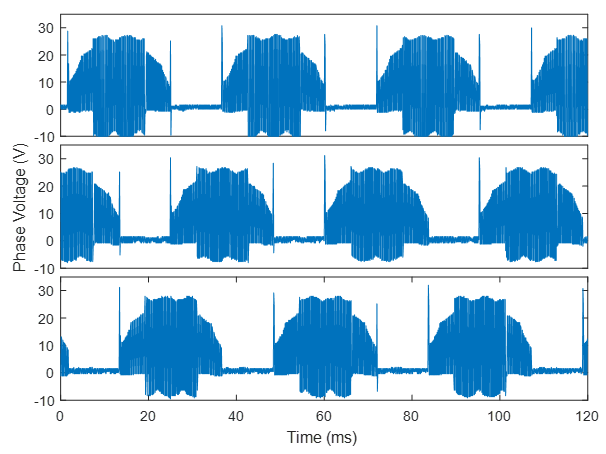
\includegraphics[width=10cm]{Images/waveforms/trap_7.png} 
\caption[trap7]{Duty Cycle = 50\%, load = 3 Nm}
\label{fig:trap7}
\end{figure}

\begin{figure}[h!p]
\centering
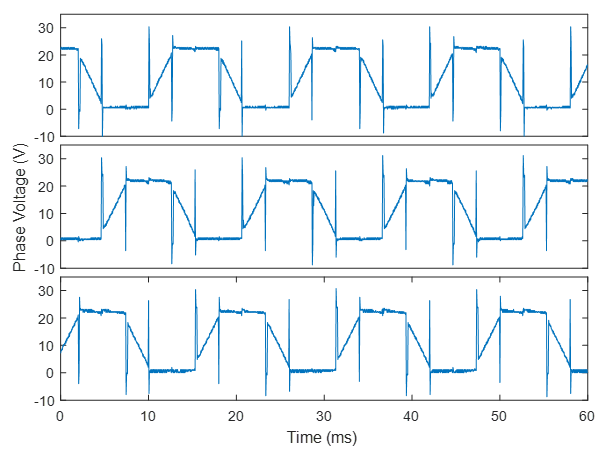
\includegraphics[width=10cm]{Images/waveforms/trap_8.png} 
\caption[trap8]{Duty Cycle = 100\%, load = 3 Nm}
\label{fig:trap8}
\end{figure}

\begin{figure}[h!p]
\centering
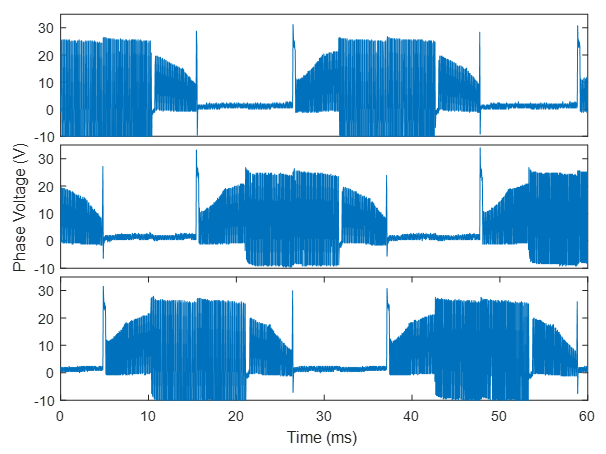
\includegraphics[width=10cm]{Images/waveforms/trap_9.png} 
\caption[trap9]{Duty Cycle = 70\%, load = 6 Nm}
\label{fig:trap9}
\end{figure}

\clearpage
\subsection{Current Waveforms}

The following images show the different current waveforms obtained according to the load applied to the motor and to the duty cycle.

\begin{figure}[h!p]
\centering
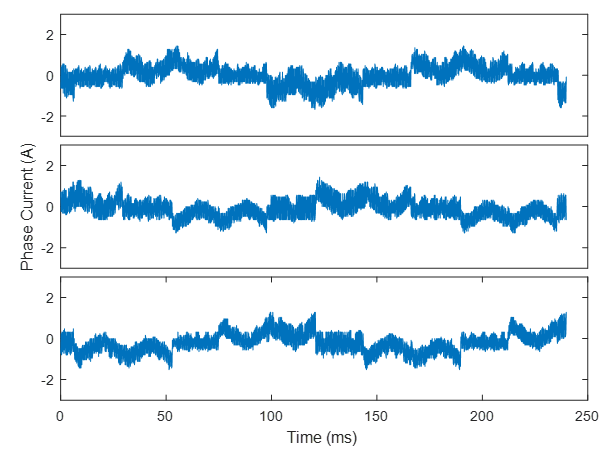
\includegraphics[width=10cm]{Images/waveforms/trap_curr_1.png}
\caption[trapc1]{Duty Cycle = 10\%, no load applied}
\label{fig:trapc1}
\end{figure}

\begin{figure}[h!p]
\centering
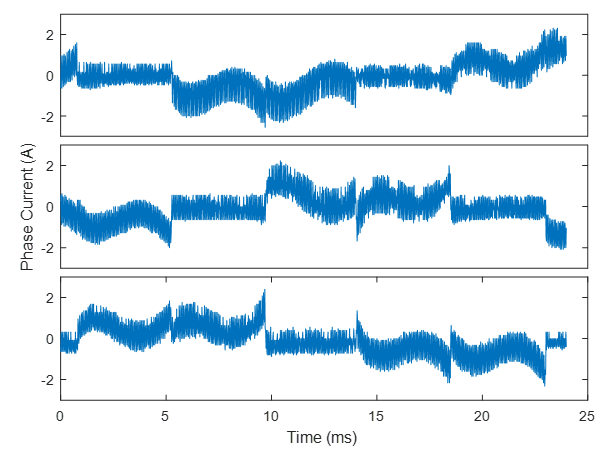
\includegraphics[width=10cm]{Images/waveforms/trap_curr_2.png} 
\caption[trapc1]{Duty Cycle = 50\%, no load applied}
\label{fig:trapc2}
\end{figure}

\begin{figure}[h!p]
\centering
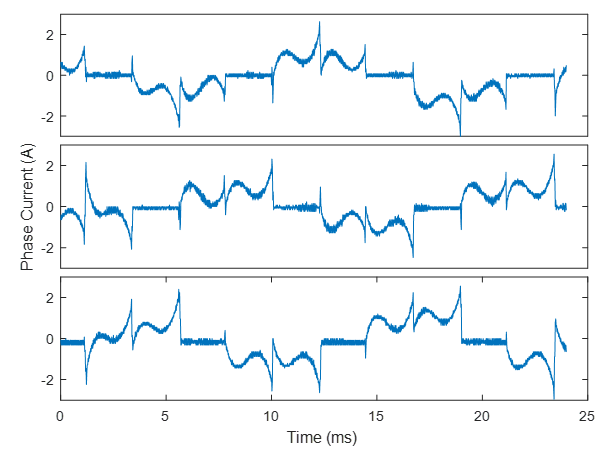
\includegraphics[width=10cm]{Images/waveforms/trap_curr_3.png} 
\caption[trapc3]{Duty Cycle = 100\%, no load applied}
\label{fig:trapc3}
\end{figure}

\begin{figure}[h!p]
\centering
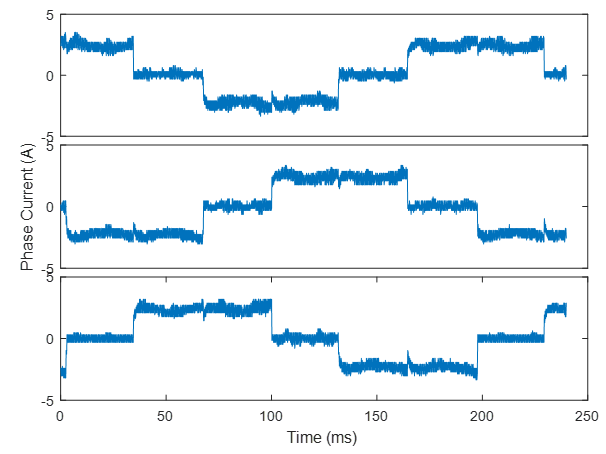
\includegraphics[width=10cm]{Images/waveforms/trap_curr_4.png} 
\caption[trapc4]{Duty Cycle = 10\%, load = 1 Nm}
\label{fig:trapc4}
\end{figure}

\begin{figure}[h!p]
\centering
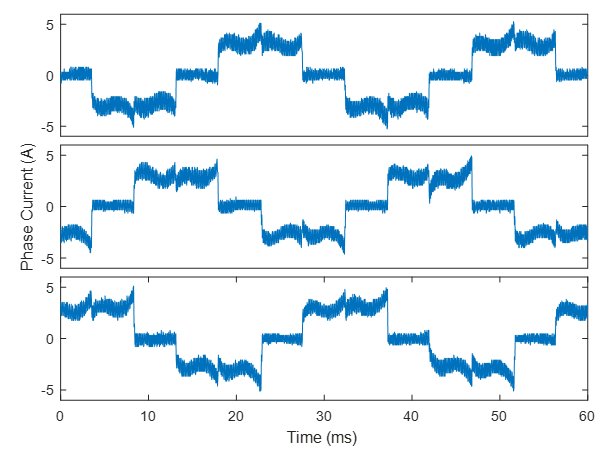
\includegraphics[width=10cm]{Images/waveforms/trap_curr_5.png} 
\caption[trapc5]{Duty Cycle = 50\%, load = 1 Nm}
\label{fig:trapc5}
\end{figure}

\begin{figure}[h!p]
\centering
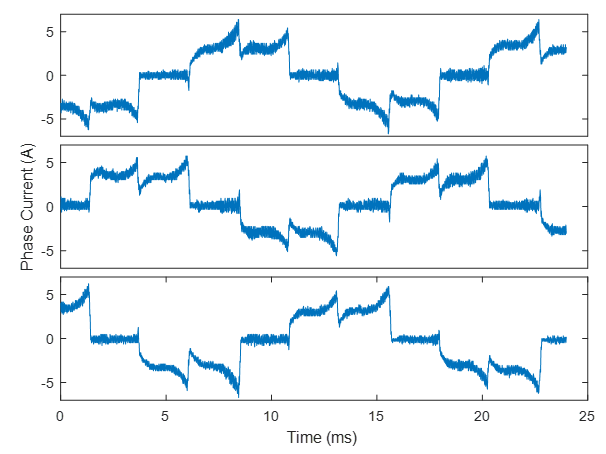
\includegraphics[width=10cm]{Images/waveforms/trap_curr_6.png} 
\caption[trapc6]{Duty Cycle = 100\%, load = 1 Nm}
\label{fig:trapc6}
\end{figure}

\begin{figure}[h!p]
\centering
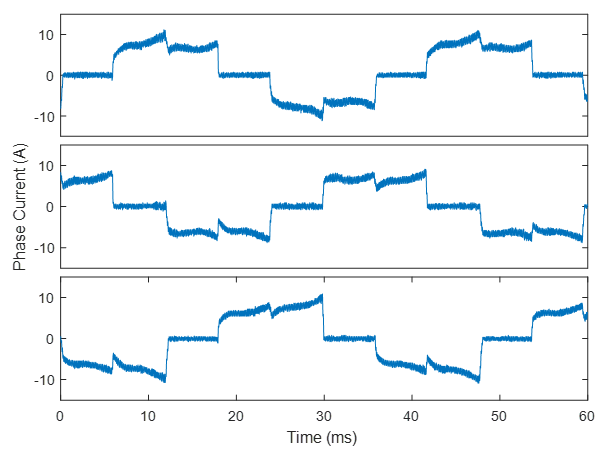
\includegraphics[width=10cm]{Images/waveforms/trap_curr_7.png} 
\caption[trapc7]{Duty Cycle = 50\%, load = 3 Nm}
\label{fig:trapc7}
\end{figure}

\begin{figure}[h!p]
\centering
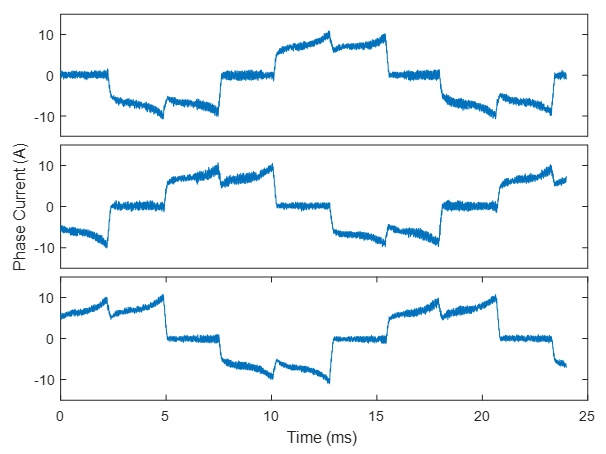
\includegraphics[width=10cm]{Images/waveforms/trap_curr_8.png} 
\caption[trapc8]{Duty Cycle = 100\%, load = 3 Nm}
\label{fig:trapc8}
\end{figure}

\begin{figure}[h!p]
\centering
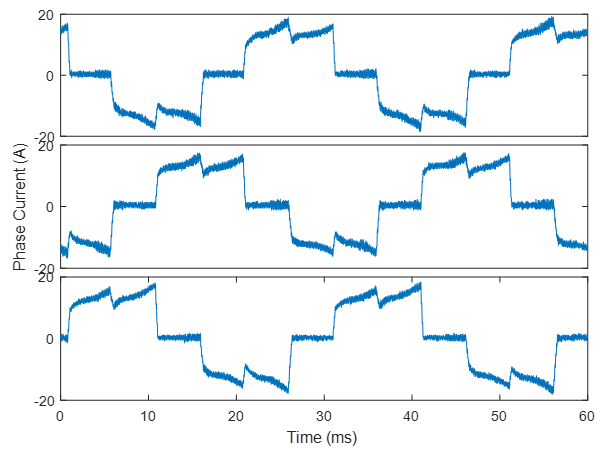
\includegraphics[width=10cm]{Images/waveforms/trap_curr_9.png} 
\caption[trapc9]{Duty Cycle = 70\%, load = 6 Nm}
\label{fig:trapc9}
\end{figure}

\clearpage
\section{Speed Control with Trapezoidal Drive}

To see the behaviour of the speed control, different unit step signals were applied with different loads and different controller parameters. 

The torque loads were setup first at a steady speed to know the correct excitation voltage of the field, then the motor was stopped and step signal was applied.

\begin{figure}[h!p]
\centering
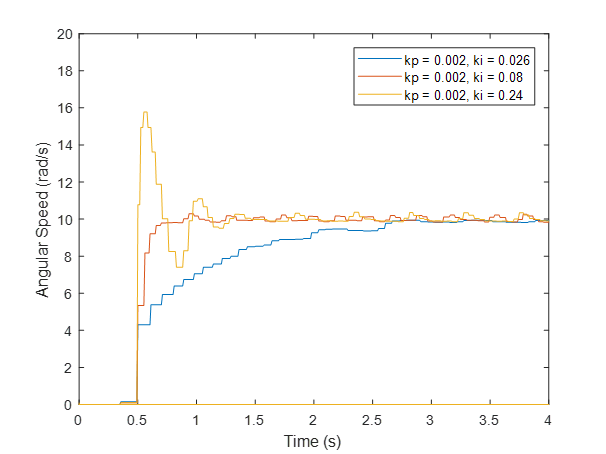
\includegraphics[width=10cm]{Images/plots/plot_2.png} 
\caption[plot2]{Step response to a 10 rad/s signal without load applied}
\label{fig:plot2}
\end{figure}

\begin{figure}[h!p]
\centering
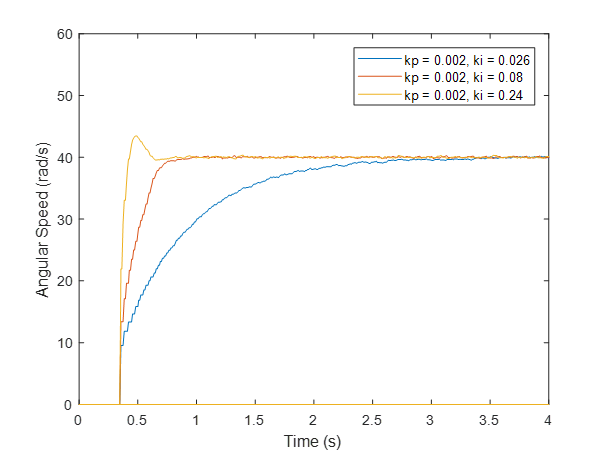
\includegraphics[width=10cm]{Images/plots/plot_3.png} 
\caption[plot3]{Step response to a 40 rad/s signal without load applied}
\label{fig:plot3}
\end{figure}

\begin{figure}[h!p]
\centering
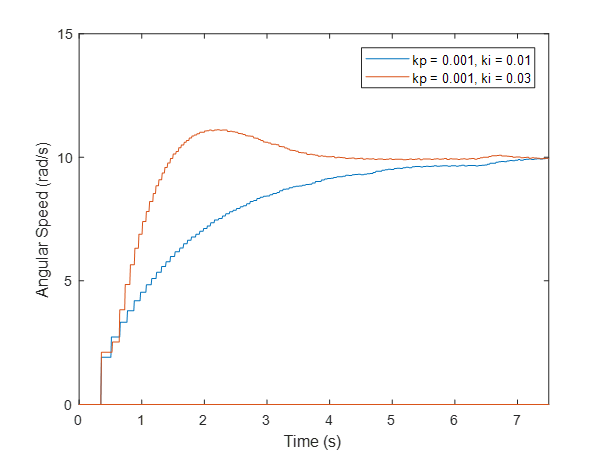
\includegraphics[width=10cm]{Images/plots/plot_4.png} 
\caption[plot4]{Step response to a 10 rad/s signal with a 3 Nm load}
\label{fig:plot4}
\end{figure}

\begin{figure}[h!p]
\centering
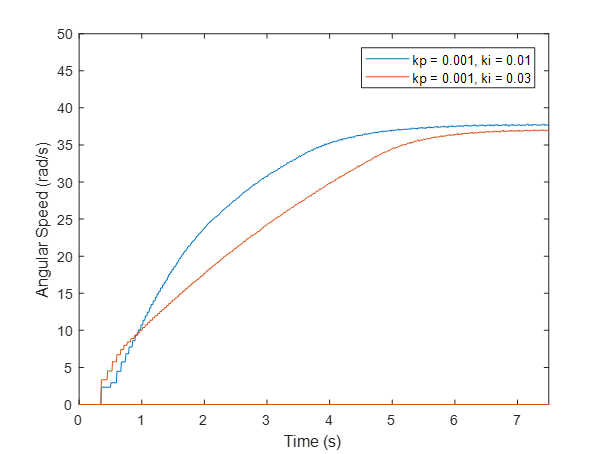
\includegraphics[width=10cm]{Images/plots/plot_5.png} 
\caption[plot5]{Step response to a 40 rad/s signal with a 3 Nm load}
\label{fig:plot5}
\end{figure}

\clearpage
It is possible to see also the speed behaviour of the system compared with the duty cycle applied by the control algorithm:

\begin{figure}[h!p]
\centering
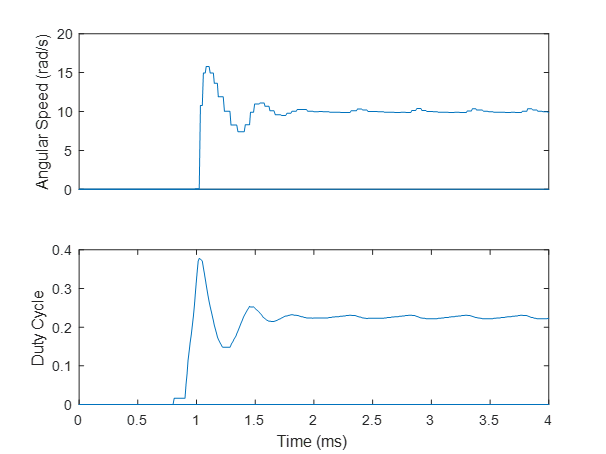
\includegraphics[width=10cm]{Images/plots/plot_6.png} 
\caption[plot6]{Step response to a 10 rad/s signal without load, compared to its driving duty cycle signal}
\label{fig:plot6}
\end{figure}

\begin{figure}[h!p]
\centering
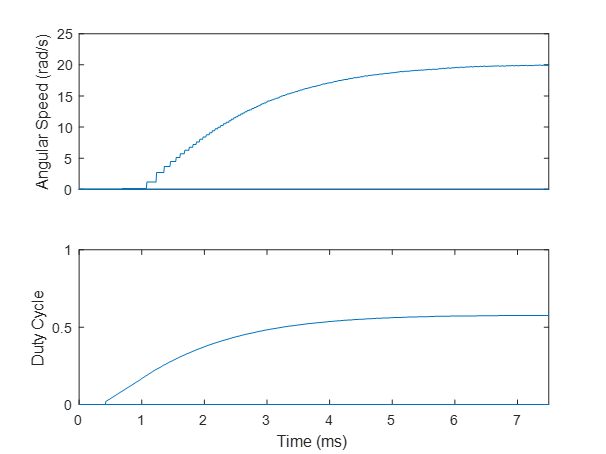
\includegraphics[width=10cm]{Images/plots/plot_7.png} 
\caption[plot7]{Step response to a 20 rad/s signal with a 3 Nm load, compared to its driving duty cycle signal}
\label{fig:plot7}
\end{figure}

\clearpage
\section{Sinusoidal Drive - Open Loop}

This test was applied at the beginning of the development of the Field Oriented Control to test the generation of a sinusoidal waveform depending on the angular position of the rotor. The signals were generated by applying a constant amplitude value.

The following images are current waveforms with different reference quadrature voltages without any load applied.

\begin{figure}[h!p]
\centering
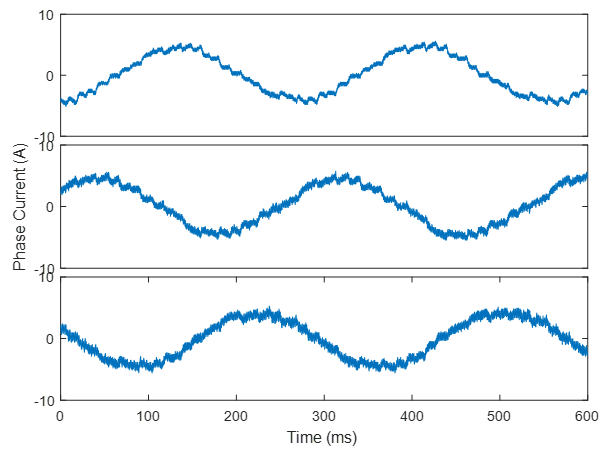
\includegraphics[width=10cm]{Images/waveforms/sin1.png} 
\caption[sin1]{Sinusoidal drive with 1 V as quadrature voltage}
\label{fig:sin1}
\end{figure}

\begin{figure}[h!p]
\centering
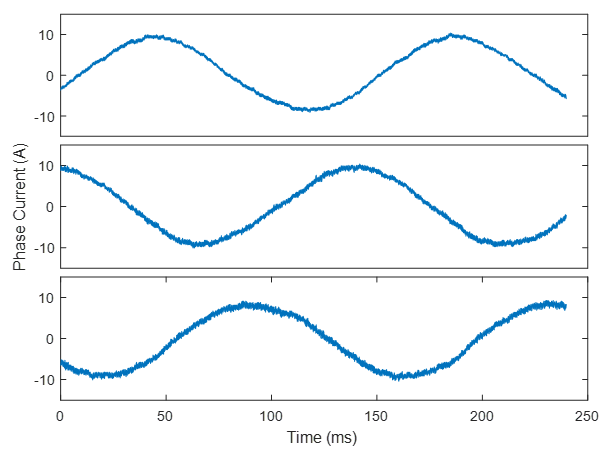
\includegraphics[width=10cm]{Images/waveforms/sin2.png} 
\caption[sin2]{Sinusoidal drive with 2 V as quadrature voltage}
\label{fig:sin2}
\end{figure}

\begin{figure}[h!p]
\centering
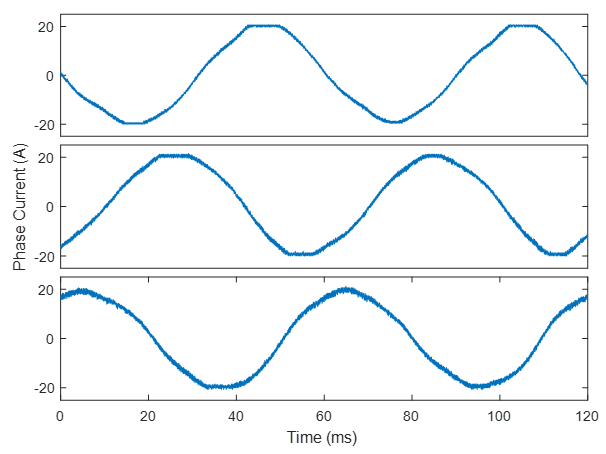
\includegraphics[width=10cm]{Images/waveforms/sin3.png} 
\caption[sin3]{Sinusoidal drive with 5 V as quadrature voltage}
\label{fig:sin3}
\end{figure}

In Figure \ref{fig:sin}, it can be appreciated that the current in the highest and lowest side of the signal are limited by the LEM current sensor of the measurement board.

\clearpage
\section{Field Oriented Control}

These tests were applied by exciting the field of the generator to the maximum available, so by setting up a reference quadrature current, the motor would reach a steady state speed when the torque applied by the load is equal to the torque applied by the motor.

\begin{figure}[h!p]
\centering
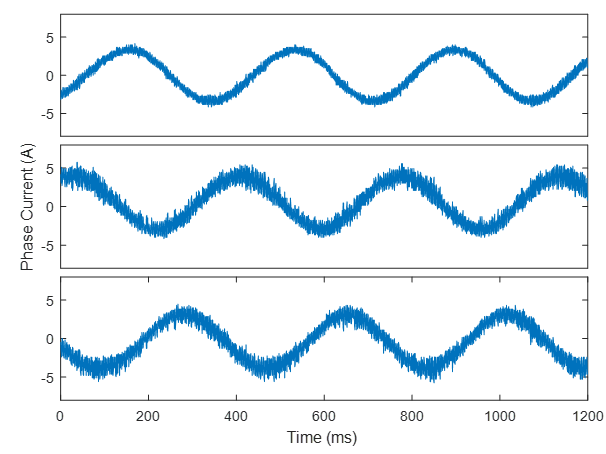
\includegraphics[width=10cm]{Images/waveforms/sin4.png} 
\caption[sin4]{FOC signal with a 1 Nm load}
\label{fig:sin4}
\end{figure}

\begin{figure}[h!p]
\centering
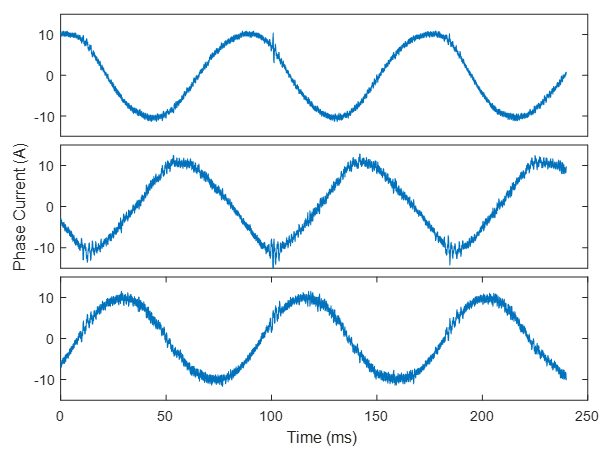
\includegraphics[width=10cm]{Images/waveforms/sin5.png} 
\caption[sin5]{FOC signal with a 3 Nm load}
\label{fig:sin5}
\end{figure}

\begin{figure}[h!p]
\centering
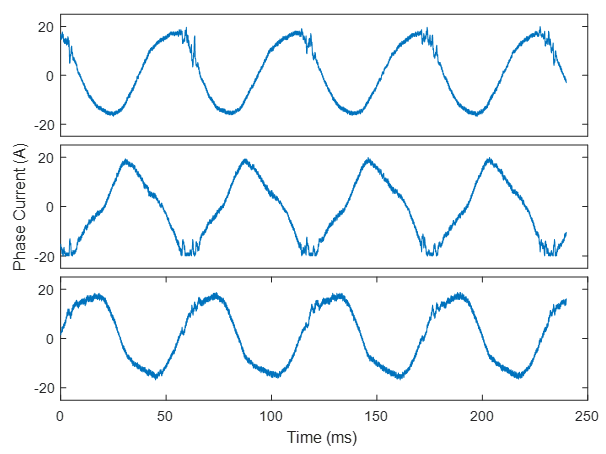
\includegraphics[width=10cm]{Images/waveforms/sin6.png} 
\caption[sin6]{FOC signal with a 5 Nm load}
\label{fig:sin6}
\end{figure}

\clearpage
\section{Speed Control with Field Oriented Control}

In the following waveforms can be appreciated the behaviour of the driver with different reference speeds and load conditions.

\begin{figure}[h!p]
\centering
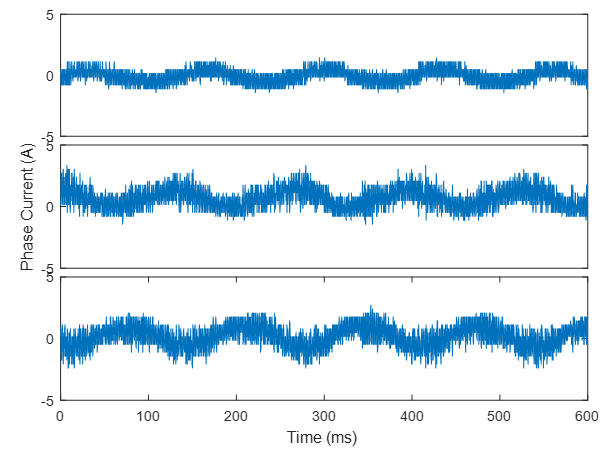
\includegraphics[width=10cm]{Images/waveforms/sin7.png} 
\caption[sin7]{5 rad/s, no load applied}
\label{fig:sin7}
\end{figure}

\begin{figure}[h!p]
\centering
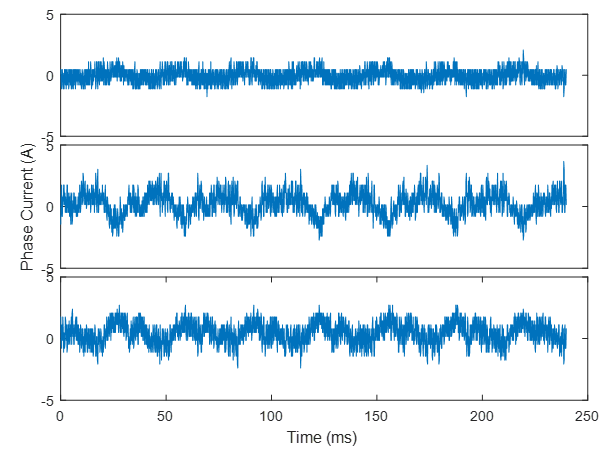
\includegraphics[width=10cm]{Images/waveforms/sin8.png} 
\caption[sin8]{20 rad/s, no load applied}
\label{fig:sin8}
\end{figure}

\begin{figure}[h!p]
\centering
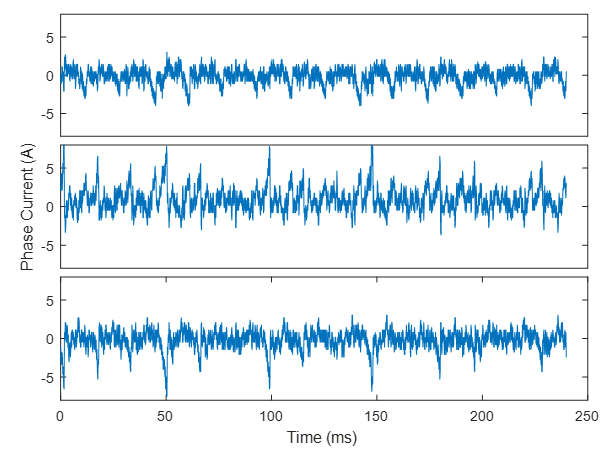
\includegraphics[width=10cm]{Images/waveforms/sin9.png} 
\caption[sin9]{40 rad/s, no load applied}
\label{fig:sin9}
\end{figure}

\begin{figure}[h!p]
\centering
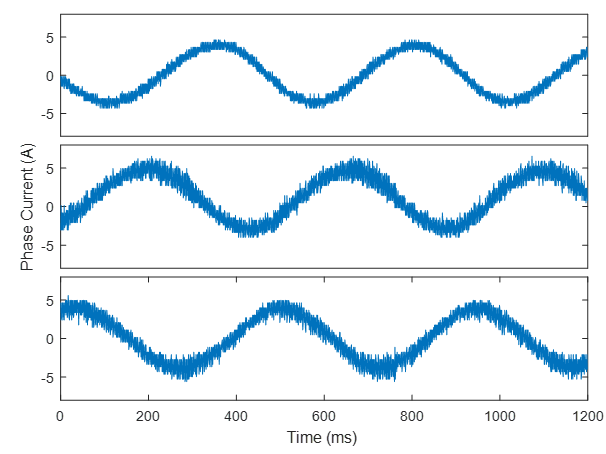
\includegraphics[width=10cm]{Images/waveforms/sin10.png} 
\caption[sin10]{1 rad/s, load = 1 Nm}
\label{fig:sin10}
\end{figure}

By analysing the frequency of the signal in Figure \ref{fig:sin10} we can see the ability of the controller to move the motor at a low speed with a load applied. It will be necessary to tune the controller parameters to drive the robot in the way that it’s needed.

\begin{figure}[h!p]
\centering
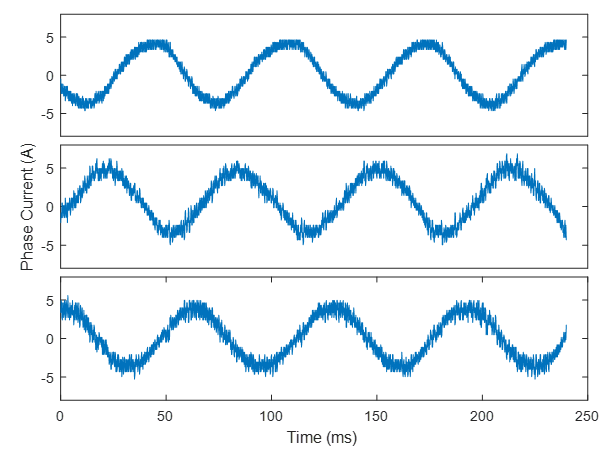
\includegraphics[width=10cm]{Images/waveforms/sin11.png} 
\caption[sin11]{10 rad/s, load = 1 Nm}
\label{fig:sin11}
\end{figure}

\begin{figure}[h!p]
\centering
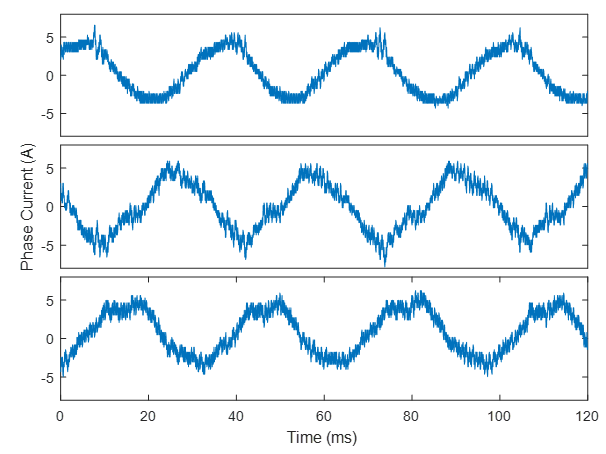
\includegraphics[width=10cm]{Images/waveforms/sin12.png} 
\caption[sin12]{20 rad/s, load = 1 Nm}
\label{fig:sin12}
\end{figure}

\begin{figure}[h!p]
\centering
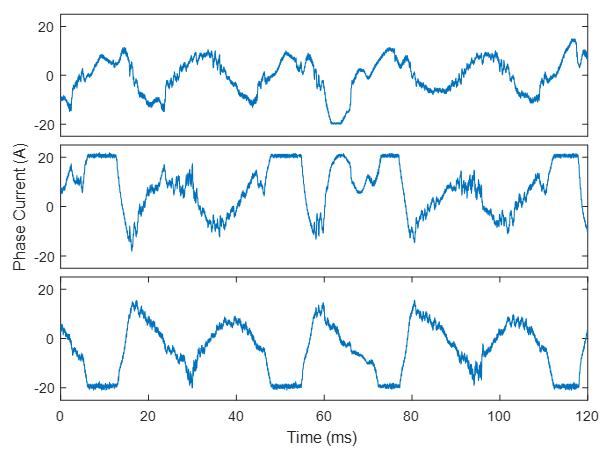
\includegraphics[width=10cm]{Images/waveforms/sin13.png} 
\caption[sin13]{30 rad/s, load = 1 Nm}
\label{fig:sin13}
\end{figure}

It can be appreciated in Figures \ref{fig:sin9}, \ref{fig:sin12} and \ref{fig:sin13} that the signal gets distorted when a certain speed is reached. This is due to the maximum frequency achievable by the angular position sensor, which limits the sampling frequency and modifies the behaviour of the controller at speeds higher than $20 rad/s$. Currently it represents a trade-off between the trapezoidal driven speed control, which works fine at high speeds since the angular position feedback is given by the hall effect sensors, and the \ac{FOC} driven speed control, which works fine at low speeds but at high speeds becomes unpredictable.

\begin{figure}[h!p]
\centering
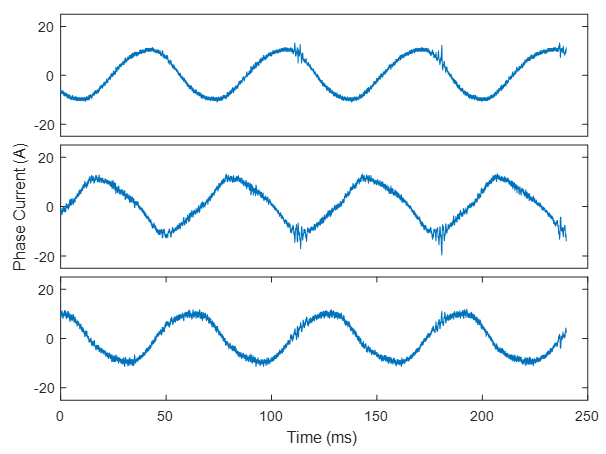
\includegraphics[width=10cm]{Images/waveforms/sin14.png} 
\caption[sin14]{10 rad/s, load = 3 Nm}
\label{fig:sin14}
\end{figure}

\begin{figure}[h!p]
\centering
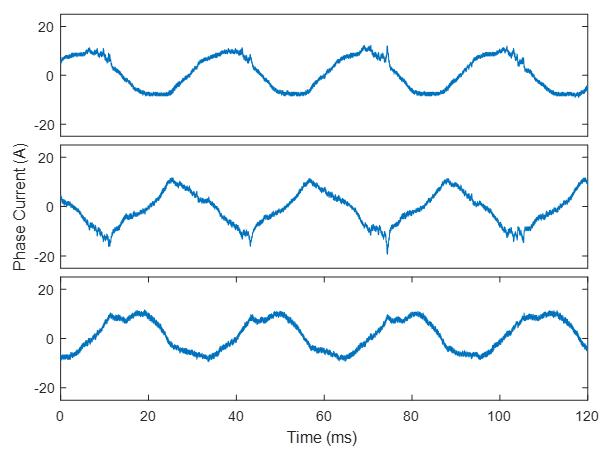
\includegraphics[width=10cm]{Images/waveforms/sin15.png} 
\caption[sin15]{20 rad/s, load = 3 Nm}
\label{fig:sin15}
\end{figure}

\clearpage

In Figure \ref{fig:plot8} we can see the comparison of the behaviour of the controller with the same step signal ($0$ to $10 rad/s$) but with different load. When the load is $3 Nm$, the slope of the signal becomes limited by the controller parameter \texttt{I\_MAX}, which defines the saturation of the integral part of the controller to avoid current peaks. This parameter can be modified accordingly to the capacities of the system, but caution must be taken since this can provoke malfunctioning of the circuit.

\begin{figure}[h!p]
\centering
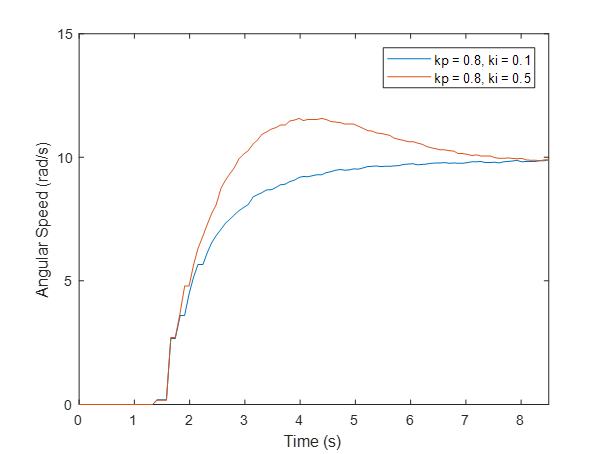
\includegraphics[width=10cm]{Images/plots/plot_8.png} 
\caption[plot8]{Step response to a 10 rad/s signal and a load of 1Nm}
\label{fig:plot8}
\end{figure}

\begin{figure}[h!p]
\centering
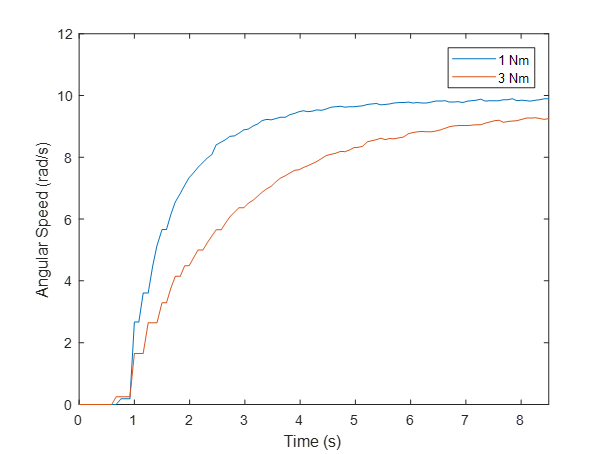
\includegraphics[width=10cm]{Images/plots/plot_9.png} 
\caption[plot9]{Step response to a 10 rad/s signal with different loads}
\label{fig:plot9}
\end{figure}

\clearpage

In the following current waveforms, we can appreciate the current settling to a steady state after a step signal is commanded to the controller.


%have these two figures in the same figure
\begin{figure}[h!p]
\centering
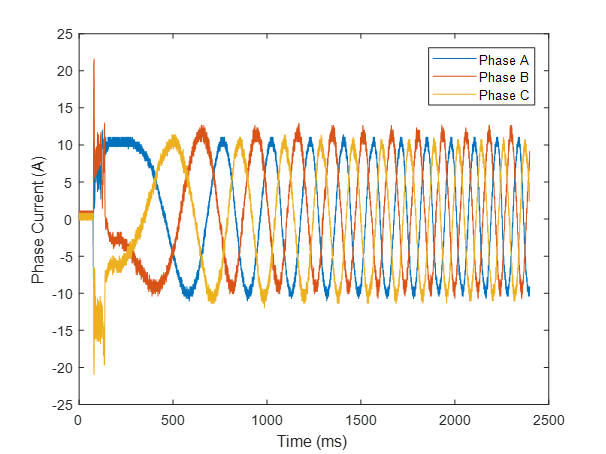
\includegraphics[width=10cm]{Images/waveforms/sin16.png} 
\caption[sin16]{Step response to 10 rad/s, load = 3 Nm}
\label{fig:sin16}
\end{figure}

\begin{figure}[h!p]
\centering
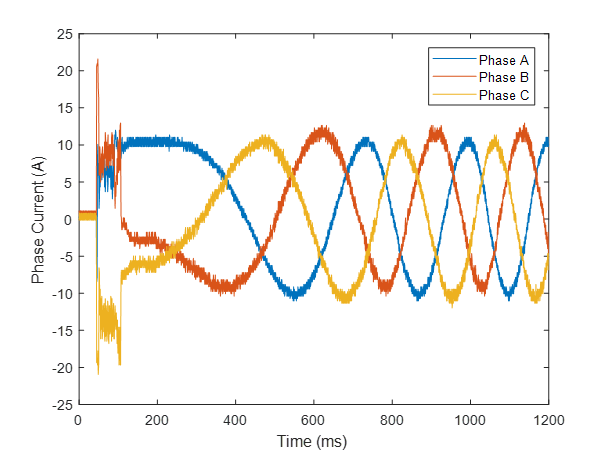
\includegraphics[width=10cm]{Images/waveforms/sin17.png} 
\caption[sin17]{Step response to 10 rad/s, load = 3 Nm}
\label{fig:sin17}
\end{figure}


%have these three figures in the same figure
\begin{figure}[h!p]
\centering
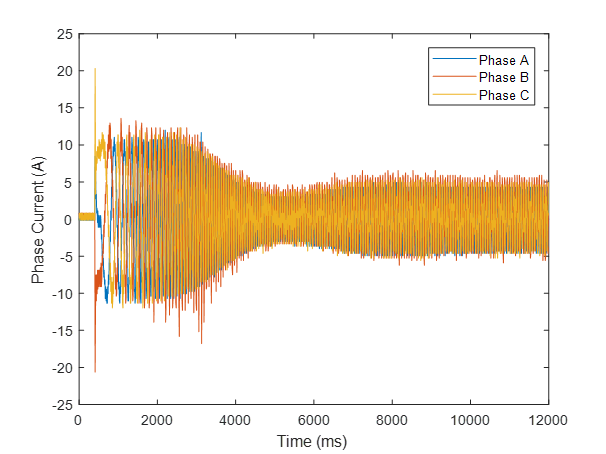
\includegraphics[width=10cm]{Images/waveforms/sin18.png} 
\caption[sin18]{Step Response 10 rad/s, Load = 1 Nm}
\label{fig:sin18}
\end{figure}

\begin{figure}[h!p]
\centering
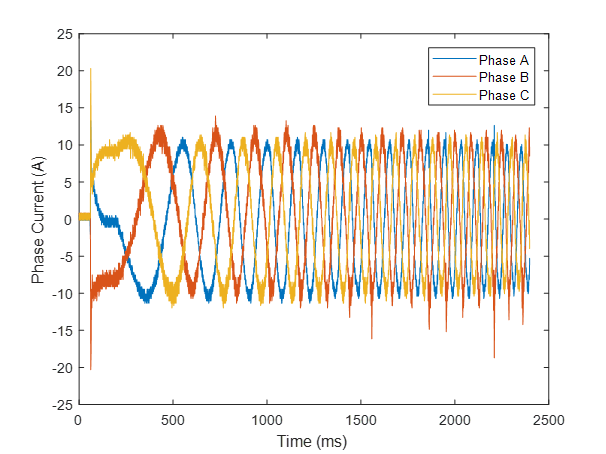
\includegraphics[width=10cm]{Images/waveforms/sin19.png} 
\caption[sin19]{Step Response 10 rad/s, Load = 1 Nm}
\label{fig:sin19}
\end{figure}

\begin{figure}[h!p]
\centering
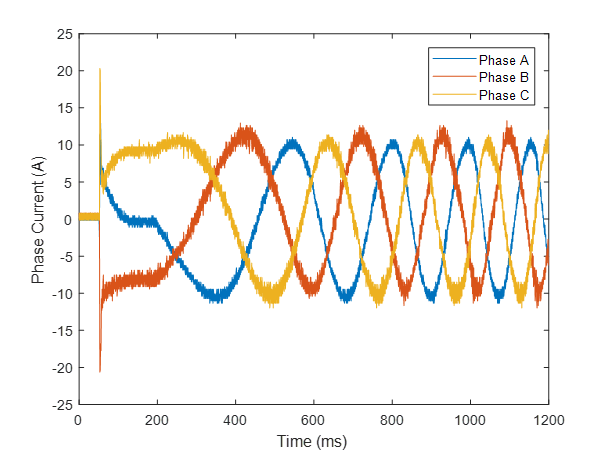
\includegraphics[width=10cm]{Images/waveforms/sin20.png} 
\caption[sin20]{Step Response 10 rad/s, Load = 1 Nm}
\label{fig:sin20}
\end{figure}